\begin{titreTice}[Généralités sur les fonctions]

\Titre{Trace active}{0}
\end{titreTice}

\vspace{0.2cm}

Très souvent la géométrie est un terrain privilégié pour introduire une fonction.
Géogébra permet de créer une figure dynamique et de mettre en évidence une courbe comme trace ou lieu de point, image d'un point mobile sur un objet (cercle, droite, segment,...)

\vspace{0.2cm}

\begin{minipage}{0.48\linewidth}
\textbf{Problème :} \textit{extrait du livre Hyperbole Seconde – Nathan 2012 }


Dans un repère d'origine $O$, $\mathscr{C}$ est le demi-cercle ci-contre de centre $O$ et de rayon 4. $A$ est le point de coordonnées (0;5). Pour tout réel $x$ de $[-4;4]$, on pose $f(x)=AM$ où $M$ est le point de $\mathscr{C}$ d'abscisse $x$.
Déterminer le tableau de variation de la fonction $f$.
\end{minipage}
\hfill
\begin{minipage}{0.48\linewidth}
\definecolor{uuuuuu}{rgb}{0.26666666666666666,0.26666666666666666,0.26666666666666666}
\definecolor{ffqqqq}{rgb}{1.,0.,0.}
\definecolor{qqqqff}{rgb}{0.,0.,1.}
\definecolor{xdxdff}{rgb}{0.49019607843137253,0.49019607843137253,1.}
\begin{tikzpicture}[line cap=round,line join=round,>=triangle 45,x=1.0cm,y=1.0cm]
\draw[->,color=black] (-4.28,0.) -- (4.5,0.);
\foreach \x in {-4.,-3.,-2.,-1.,1.,2.,3.,4.}
\draw[shift={(\x,0)},color=black] (0pt,2pt) -- (0pt,-2pt) node[below] {\footnotesize $\x$};
\draw[->,color=black] (0.,-0.58) -- (0.,5.44);
\foreach \y in {,1.,2.,3.,4.,5.}
\draw[shift={(0,\y)},color=black] (2pt,0pt) -- (-2pt,0pt);
\draw[color=black] (0pt,-10pt) node[right] {\footnotesize $0$};
\clip(-4.28,-0.58) rectangle (4.5,5.44);
\draw [shift={(0.,0.)}] plot[domain=0.:3.141592653589793,variable=\t]({1.*4.*cos(\t r)+0.*4.*sin(\t r)},{0.*4.*cos(\t r)+1.*4.*sin(\t r)});
\draw [color=ffqqqq] (-2.4141512871263906,3.18933748024037)-- (0.,5.);
\draw [color=ffqqqq] (-2.4141512871263906,3.18933748024037)-- (-2.4141512871263906,0.);
\draw (-2.54,0.12) node[anchor=north west] {$x$};
\begin{scriptsize}
\draw [fill=xdxdff] (-4.,0.) circle (2.5pt);
\draw[color=xdxdff] (-3.86,0.36) node {$B$};
\draw [fill=qqqqff] (4.,0.) circle (2.5pt);
\draw[color=qqqqff] (4.14,0.36) node {$C$};
\draw [fill=xdxdff] (0.,5.) circle (2.5pt);
\draw[color=xdxdff] (0.14,5.36) node {$A$};
\draw [fill=xdxdff] (-2.4141512871263906,3.18933748024037) circle (2.5pt);
\draw[color=xdxdff] (-2.86,3.4) node {$M$};
\draw [fill=uuuuuu] (-2.4141512871263906,0.) circle (1.5pt);
\end{scriptsize}
\end{tikzpicture}

\end{minipage}

\vspace{0.2cm}

\textbf{Étape 1} : Dans la fenêtre graphique 1, on construit la figure avec le point $M$ sur l'objet cercle.

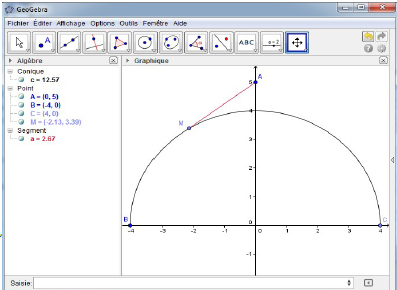
\includegraphics[scale=0.5]{VF-F2-0.jpg}

Pour tracer cette figure, on utilise les icônes
\begin{description}
    \item[•] 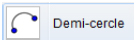
\includegraphics[scale=0.5]{VF-F2-20.jpg} 
    \item[•] 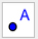
\includegraphics[scale=0.5]{VF-F2-21.jpg}  pour placer le point M sur le demi cercle
\end{description}       
        
Créer le segment AM : dans la fenêtre algèbre la longueur AM est notée $a$.

\vspace{0.2cm}

\textbf{Étape 2 :}  Ouvrir la fenêtre graphique 2

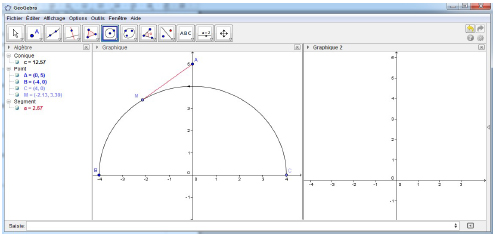
\includegraphics[scale=0.5]{VF-F2-1.jpg} 

\vspace{0.2cm}

\textbf{Etape 3 :} Rendre la fenêtré graphique 2 active. Au besoin, cliquez simplement sur la fenêtre graphique 2. Graphique 2 se met en gras et Graphique 1 en normal.

\vspace{0.2cm}

Dans la barre de saisie, créer le point $N=(x(M),a)$. 
Attention entre les 2 coordonnées du point $M$, il faut écrire une virgule et non un point-virgule sinon le point $M$ est placé selon ses coordonnées polaires.
$x(M)$ est l'instruction Géogébra qui donne l'abscisse du point $M$.

\vspace{0.2cm}

\textbf{Étape 4 :}

\vspace{0.2cm}

\begin{minipage}{0.68\linewidth}
Cliquez droit sur le point $N$ ou cliquez le point $N$ dans la fenêtre algèbre. Une fenêtre contextuelle apparaît et propose les propriétés du point $N$.
Ouvrir les propriétés de $N$.
Dans l'onglet « Basique », cochez « afficher la trace ».
Puis fermez la fenêtre contextuelle.
\end{minipage}
\hfill
\begin{minipage}{0.28\linewidth}

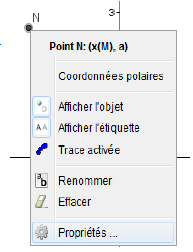
\includegraphics[scale=0.5]{VF-F2-5.jpg} 

\end{minipage}
\vspace{0.2cm}

\textbf{Étape 5 }: Trace du point $N$

\vspace{0.2cm}

A l'aide de l’icône  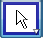
\includegraphics[scale=0.5]{VF-F2-4.jpg}         déplacer le point $M$ dans la fenêtre Graphique 1. La trace du point $N$ apparaît sur la fenêtre Graphique 2.

On peut automatiser la situation en animant le point M dans la fenêtre contextuelle du point $M$, Dans l'onglet « Basique », cochez «animer ». et mettre en relief la position de M en affichant sa trace active.

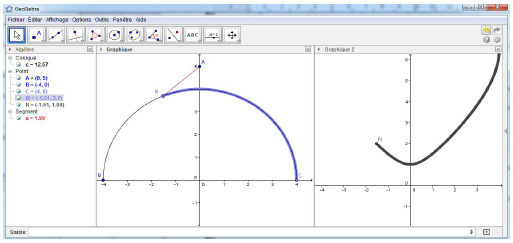
\includegraphics[scale=0.5]{VF-F2-6.jpg} 